% Copyright 2026  Ed Bueler

\documentclass[10pt,
               svgnames,
               hyperref={colorlinks,
                         citecolor=DeepPink4,
                         linkcolor=FireBrick,
                         urlcolor=blue},
               usepdftitle=false]{beamer}

\usetheme{Madrid}
\usecolortheme{beaver}
\setbeamercovered{transparent}
\setbeamerfont{frametitle}{size=\large}
\setbeamercolor*{block title}{bg=red!10}
\setbeamercolor*{block body}{bg=red!5}

\usepackage[english]{babel}
\usepackage[latin1]{inputenc}
\usepackage{times}
\usepackage[T1]{fontenc}
% Or whatever. Note that the encoding and the font should match. If T1
% does not look nice, try deleting the line with the fontenc.

\usepackage{fancyvrb,empheq,bm,xspace,dsfont}
\usepackage{minted}
\usepackage{tikz}

% If you wish to uncover everything in a step-wise fashion, uncomment
% the following command: 
%\beamerdefaultoverlayspecification{<+->}

\newcommand{\bb}{\mathbf{b}}
\newcommand{\bc}{\mathbf{c}}
\newcommand{\bbf}{\mathbf{f}}
\newcommand{\bl}{\bm{\ell}}
\newcommand{\br}{\mathbf{r}}
\newcommand{\bs}{\mathbf{s}}
\newcommand{\bx}{\mathbf{x}}
\newcommand{\by}{\mathbf{y}}
\newcommand{\bv}{\mathbf{v}}
\newcommand{\bu}{\mathbf{u}}
\newcommand{\bw}{\mathbf{w}}

\newcommand{\bzero}{\bm{0}}

\newcommand{\cE}{\mathcal{E}}
\newcommand{\cF}{\mathcal{F}}
\newcommand{\cM}{\mathcal{M}}
\newcommand{\cR}{\mathcal{R}}

\newcommand{\CC}{\mathbb{C}}
\newcommand{\NN}{\mathbb{N}}
\newcommand{\QQ}{\mathbb{Q}}
\newcommand{\RR}{\mathbb{R}}
\newcommand{\ZZ}{\mathbb{Z}}

\newcommand{\one}{\mathds{1}}

\newcommand{\stri}{\mathbin{\triangle}}

\newcommand{\range}{\operatorname{range}}
\newcommand{\Span}{\operatorname{span}}

\newcommand{\Matlab}{\textsc{Matlab}\xspace}
\newcommand{\eps}{\epsilon}

\newcommand{\ds}{\displaystyle}

\newcommand{\ip}[2]{\left<#1,#2\right>}

\newcommand{\twovect}[4]{\ensuremath{{#1}_{#2} =
                            \begin{bmatrix} #3 \\ #4 \end{bmatrix}}}

\newcommand{\rbullet}{{\color{FireBrick} \bullet}}

\newcommand*\circled[1]{\tikz[baseline=(char.base)]{
            \node[shape=circle,draw,inner sep=2pt] (char) {#1};}}

\newcommand{\textbook}{Saxe, \emph{Beginning Functional Analysis}}

\DefineVerbatimEnvironment{mVerb}{Verbatim}{numbersep=2mm,
frame=lines,framerule=0.1mm,framesep=2mm,xleftmargin=4mm,fontsize=\scriptsize}

\newcommand{\itemnum}[1]{\setcounter{enumi}{#1}\usebeamertemplate{enumerate item}}



\title{Functions defined in pieces: \\ simple, step, and piecewise-linear}

\subtitle{a calculation for week 6}

\author{Ed Bueler}

\institute[]{UAF Math 617 Functional Analysis}

\date{Spring 2026}


\begin{document}
\beamertemplatenavigationsymbolsempty

\begin{frame}
  \maketitle
\end{frame}


\begin{frame}{Outline}
  \tableofcontents[hideallsubsections]
\end{frame}

\AtBeginSection[]
{% do not put toc here this time
}


\section{measurable subsets of $\RR^1$, and Lebesgue measure}

\begin{frame}{intervals and their lengths}

\begin{itemize}
\item in Chapter 3 our textbook defines \emph{measurable subset} (of $\RR^n$), and then \emph{simple function} (from $\RR^n$ to $\RR$)
\item I will give the definitions for $\RR^1$ here
\end{itemize}

\begin{definition}
\begin{itemize}
\item for real numbers $a\le b$, a \emph{finite interval} $I\subset \RR^1$ is either
    $$(a,b) \text{ or } (a,b] \text{ or } [a,b) \text{ or } [a,b]$$ 
\item the \emph{length} of a (finite) interval is
    $$m(I) = b - a < \infty$$
\end{itemize}
\end{definition}

\begin{itemize}
\item singleton sets, and the empty set, are finite intervals with length zero
   \begin{itemize}
   \item[$\circ$] $\{a\} = [a,a]$ and $\emptyset = (a,a)$
   \end{itemize}
\end{itemize}
\end{frame}


\begin{frame}{outer measure}

\begin{definition}
for any subset $A\subset \RR^1$, the \emph{outer measure} is
	$$m^*(A) = \inf\, \left\{\sum_{k=1}^\infty m(I_k)\,:\,A \subset \bigcup_{k=1}^\infty I_k\right\}$$
where the infimum is over countable unions of (finite) intervals $I_k$ covering $A$
\end{definition}

\begin{itemize}
\item $m^*(A)$ is defined for \emph{any} subset $A\subset \RR^1$
\item thus $m^* : 2^{(\RR^1)} \to [0,+\infty]$
   \begin{itemize}
   \item[$\circ$] the \emph{power set} of a set $S$ is \, $2^S = \left\{A \,:\, A\subset S\right\}$
   \end{itemize}
\item $m^*(A)=+\infty$ if there is no open covering of $A$ by countably-many intervals of finite total length
\end{itemize}
\end{frame}


\begin{frame}{outer measure: examples}
\begin{itemize}
\item[Ex 1] if $I$ is any interval then $m^*(I)$ is the length of $I$
   \begin{itemize}
   \item[$\circ$] $m^*(\RR)=+\infty$, and likewise for half-infinite intervals like $[a,+\infty)$
   \end{itemize}
\item[Ex 2] if $A$ is a finite or countable set then $m^*(A)=0$

\begin{proof}
\phantom{x}

\vspace{15mm}
\end{proof}
\item[Ex 3] $m^*(\QQ)=0$
\item[Ex 4] $m^*(C)=0$ where $C \subset [0,1]$ is the \emph{Cantor middle-thirds set}  \hfill [\emph{picture}]

\vspace{14mm}
\item[Ex 5] $m^*([0,1]\setminus\QQ)=1$ and $m^*(\RR\setminus\QQ)=+\infty$
\end{itemize}
\end{frame}


\begin{frame}{measure zero}

\begin{definition}
a subset $A\subset \RR^1$ has \emph{measure zero} if $m^*(A)=0$
\end{definition}

\begin{lemma}
$A\subset \RR^1$ has measure zero if and only if for every $\eps>0$ there is a countable covering of $A$ by intervals of total length less than $\eps$:
	$$\sum_{k=1}^\infty m(I_k) < \eps \qquad \text{ where } A \subset \bigcup_{k=1}^\infty I_k$$
\end{lemma}

{\small \noindent \emph{Proof.}
Just think through the definition of $m^*(A)=0$.  \qed
}

\bigskip
\begin{itemize}
\item every subset of a measure zero set has measure zero
\item every finite or countable set has measure zero
\item the Cantor set $C\subset[0,1]$, though it has uncountable cardinality, has measure zero
\end{itemize}
\end{frame}


\begin{frame}{certain subsets of $\RR^1$?}

\begin{definition}
given two sets $A,B$, their \emph{symmetric difference} is the set
	$$S(A,B) = (A \setminus B) \cup (B \setminus A) = (A \cup B) \setminus (A\cap B)$$
\end{definition}

\begin{definition}
section 3.2 defines three collections of subsets of $\RR^1$:
\begin{itemize}
\item {\large $\cE$} is the collection of finite, disjoint unions of (finite) intervals
\item {\large $\cM_\cF$} is the collection of all $A\subset \RR^1$ such that
	$$m^*(S(A_k,A)) \to 0 \text{ as } k \to \infty$$
for some sequence $A_k \in \cE$
\item {\large $\cM$} is the collection of finite and countable unions of sets from $\cM_\cF$
\end{itemize}
\end{definition}

\vspace{-2mm}

{\large
	$$\cE \subset \cM_{\cF} \subset \cM \subset 2^{(\RR^1)}$$
}
\end{frame}


\begin{frame}{Lebesgue measurable subsets of $\RR^1$}

\begin{definition}
$\cM$ is the collection of \emph{Lebesgue measurable sets}
\end{definition}

\begin{itemize}
\item every interval is measurable: $I \in \cM$
\item every finite union of intervals is measurable: $\cE \subset \cM$
\item every set of measure zero is measurable
\item every measurable set can be well-approximated by a countable, disjoint union of intervals:
	$$A \in \cM \iff \forall \eps>0\, \exists\, B=\bigcup_{k=1}^\infty I_k \text{ so that } m^*(S(A,B))<\eps$$
\item<2> \alert{there exist $A\subset \RR^1$ that are not Lebesgue measurable}:
   $$\cM \subsetneq 2^{(\RR^1)}$$
\item<2> more on measurable sets in Chapter 3
\end{itemize}
\end{frame}


\begin{frame}{two very useful lemmas}

\begin{lemma}
$G \subset \RR^1$ is open if and only if it is a countable, disjoint union of open intervals:
	$$G = \bigcup_{k=1}^\infty (a_k, b_k) \qquad \text{ where } a_k,b_k \in [-\infty,+\infty]$$
\end{lemma}

\begin{itemize}
\item thus $m^*(G) = \sum_{k} b_k - a_k$ for open sets $G$
\end{itemize}

\begin{lemma}
a measurable set can be squeezed between a closed and an open set:
	$$A \in \cM \qquad \iff \qquad \begin{matrix} \forall \eps>0 \, \exists E \text{ closed } \, \exists G \text{ open } \text{ s.t. } \hspace{10mm} \\ E \subset A \subset G\, \text{ and }\, m^*(G\setminus E)<\eps \end{matrix}$$
\end{lemma}

\noindent picture:

\vspace{13mm}
\end{frame}


\begin{frame}{but what is ``Lebesgue measure''?}

\begin{definition}
\emph{Lebesgue measure} is the function $m:\cM \to [0,+\infty]$ defined as the outer measure restricted to the measurable sets:
\begin{align*}
m : \cM &\to [0,+\infty] \\
    A &\mapsto m^*(A)
\end{align*}
\end{definition}

\begin{itemize}
\item what's the key property of a measure? \emph{countable additivity}
\end{itemize}

\begin{lemma}
if $A_k\in \cM$ are pairwise disjoint ($A_j \cap A_k = \emptyset$ if $j\ne k$) then
	$$m\left(\bigcup_{k=1}^\infty A_k\right) = \sum_{k=1}^\infty m(A_k)$$
\end{lemma}
\end{frame}


% at start of sections 2,3,... put outline
\AtBeginSection[] {
    \begin{frame}{Outline}
    \setbeamertemplate{section in toc}[sections numbered]
    \tableofcontents[currentsection]%,hideallsubsections]
    \end{frame}
}

\section{simple functions}

\begin{frame}{simple functions}

\begin{definition}
the \emph{indicator function} for the set $A\subset \RR^1$ is
	$$\one_A(x) = \begin{cases} 1, & x\in A \\ 0, & x\notin A \end{cases}$$
\end{definition}

\begin{itemize}
\item also denoted $\chi_A(x)$
\end{itemize}

\begin{definition}
a \emph{simple function}, $s:\RR^1\to\RR$, is a finite linear combination of indicator functions of measurable sets $E_k \in \cM$, using coefficients $c_k\in\RR$:
	$$s(x) = \sum_{k=1}^N c_k \one_{E_k}(x)$$
\end{definition}
\end{frame}


\begin{frame}{integrals of simple functions}

\begin{itemize}
\item the integral of a simple function \, $\ds s(x) = \sum_{k=1}^N c_k \one_{E_k}(x)$ \, is obvious?
\item assume $\sum_k m(E_k)<\infty$ for simplicity
\end{itemize}

\begin{definition}
if $s$ is a measurable simple function then its \emph{Lebesque integral} is
	$$\int_\RR s(x)\,dx = \sum_{k=1}^N c_k m(E_k)$$
\end{definition}

\noindent picture:

\vspace{35mm}
\end{frame}


\begin{frame}{the fundamental idea of Lebesgue integrals}

\begin{itemize}
\item \textbf{idea:} cut-up the \emph{range} of $f:[a,b] \to \RR$, and approximate by a simple function, and integrate that simple function
   \begin{itemize}
   \item[$\circ$] $f$ has to be \emph{measurable} \hfill \alert{$\longleftarrow$ to define!}
   \end{itemize}
\item the range is cut into $y_0<y_1<\dots<y_N$:
	$$s(x) = \sum_{k=0}^{N-1} y_{k}\, \one_{f^{-1}([y_{k},y_{k+1}))}(x)$$

   \begin{itemize}
   \item[$\circ$] $E_k = f^{-1}([y_{k},y_{k+1}))$ are the measurable sets for this simple function
   \end{itemize}
\end{itemize}

\begin{definition}[nearly the right definition]
for a measurable $f:[a,b] \to \RR$, the \emph{Lebesgue integral} is
    $$\int_a^b f(x)\,dx = \lim_{N\to \infty} \sum_{k=0}^{N-1} y_{k}\, m\left(f^{-1}([y_{k},y_{k+1}))\right)$$
\end{definition}
\end{frame}


\begin{frame}{the fundamental idea of Lebesgue integrals}

\begin{definition}
for a measurable $f:[a,b] \to \RR$, the \emph{Lebesgue integral} is
    $$\int_a^b f(x)\,dx = \lim_{N\to \infty} \sum_{k=0}^{N-1} y_{k}\, m\left(f^{-1}([y_{k},y_{k+1}))\right)$$
\end{definition}

\noindent picture:

\vspace{70mm}
\end{frame}


\section{step functions ($=$ piecewise-constant)}

\begin{frame}{step functions on 1D meshes}

\begin{itemize}
\item simple functions $\ds s(x) = \sum_{k=1}^N c_k \one_{E_k}(x)$ are as complicated as the sets $E_k$
    \begin{itemize}
    \item[$\circ$] measurable sets $E_k$ can be quite intricate, e.g.~Cantor sets
    \end{itemize}
\item what if we restrict $E_k$ to be intervals?
\item given a 1D mesh $x_0<x_1<x_2<\dots<x_n$, define the (finite) intervals to be $I_k=[x_{k-1},x_k]$ or $[x_{k-1},x_k)$ or $(x_{k-1},x_k]$ or $(x_{k-1},x_k)$
\end{itemize}

\begin{definition}[equivalent forms]
\begin{itemize}
\item given $x_0<x_1<x_2<\dots<x_n$ and $c_k \in \RR$ a \emph{step function} is
     $$q(x) = \sum_{k=1}^N c_k \one_{I_k}(x)$$
\item a simple function is a \emph{step function} if each $E_k$ is a finite interval
\end{itemize}
\end{definition}
\end{frame}


\begin{frame}{the two integrals (rough idea)}

\begin{itemize}
\item simple functions $\leftrightarrow$ Lebesgue integrals
\item step functions $\leftrightarrow$ Riemann integrals
\end{itemize}

\begin{block}{integration concepts}
\begin{itemize}
\item approximate $f:[a,b] \to \RR$ by simple functions, integrate those using the Lebesgue measure, and take a limit to get the \emph{Lebesgue integral}:
    $$\int_a^b f(x)\,dx = \lim_{N\to \infty} \sum_{k=0}^{N-1} y_{k}\, m\left(f^{-1}([y_{k},y_{k+1}))\right)$$
\item approximate $f:[a,b] \to \RR$ by step functions, integrate those, and take a limit to get the \emph{Riemann integral}:
    $$\int_a^b f(x)\,dx = \lim_{N\to \infty} \sum_{k=0}^{N-1} f(x_k^*)\, (x_k-x_{k-1})$$
\end{itemize}
\end{block}
\end{frame}


\section{piecewise-linear functions}

\begin{frame}{foo}

\begin{block}{x}
y
\end{block}
\end{frame}


\section{piecewise functions on triangles (\emph{first look at finite elements})}

\begin{frame}[fragile]
\frametitle{foo}

\inputminted[fontsize=\small]{python}{codes/triangles.py}

\begin{block}{x}
y
\end{block}
\end{frame}


\begin{frame}{piecewise-linear (and piecewise-constant) on a 2D mesh}

\begin{columns}
\begin{column}{0.4\textwidth}
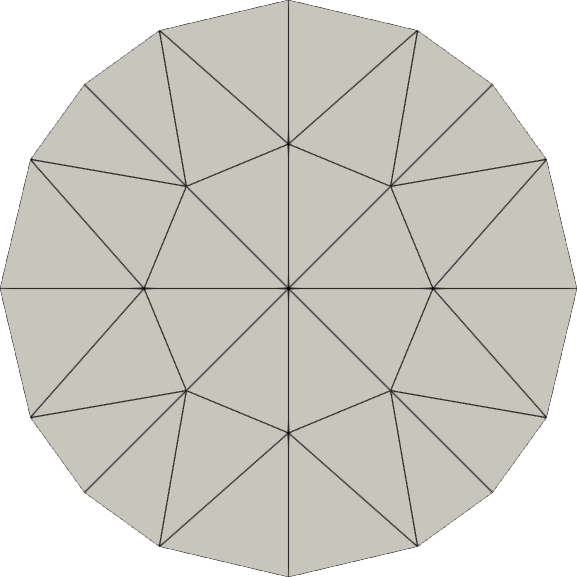
\includegraphics[width=0.8\textwidth]{figs/mesh.png}

mesh of triangles

\bigskip
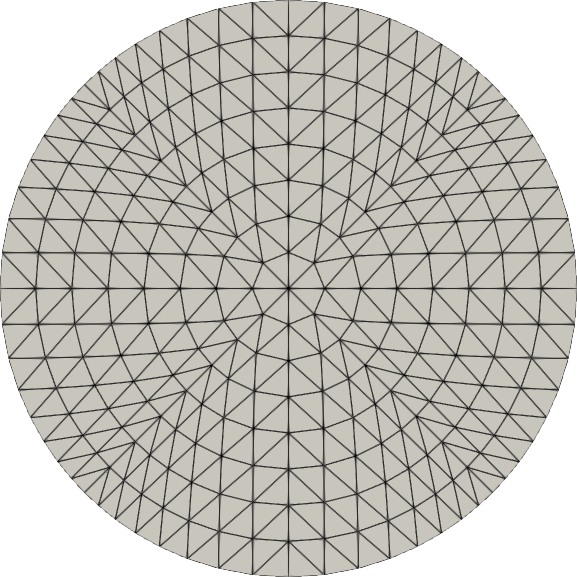
\includegraphics[width=0.55\textwidth]{figs/meshfine.png}

refined mesh
\end{column}
\begin{column}{0.6\textwidth}
\hfill \includegraphics<1>[width=0.75\textheight]{figs/dome.png}\includegraphics<2>[width=0.8\textheight]{figs/DGdome.png}\includegraphics<3>[width=0.8\textheight]{figs/DGdomefine.png}

\bigskip

\hfill \only<1>{piecewise-linear interpolant of}\only<2-3>{piecewise-constant interpolant of}

\hfill $f(x,y) = 1 - x^2 - y^2$
\end{column}
\end{columns}
\end{frame}



\section{theory from the book}

\begin{frame}{theory in week 6: Chapter 3 in Saxe}

\begin{block}{to define:}
\begin{itemize}
\item \emph{ring} of sets, and \emph{$\sigma$-ring} of sets $\cR$ \hfill ($=$ \emph{algebra} and $\sigma$-\emph{algebra})
\item an abstract \emph{measure} $\mu$
\item \emph{Lebesgue outer measure} $m^*$ on $\RR^n$
\item \emph{Lebesgue measurable} subsets $\cM$ of $\RR^n$
\item \emph{Lebesgue measure} $m$
\item \emph{simple functions} and their integrals
\item $f:\RR^n\to \RR$ is \emph{measurable}
\item \emph{Lebesgue integral} $\int_E f\,dm$
\item abstract/general: \emph{measure space} $(X,\cR,\mu)$, \emph{measurable} $f:X\to \RR$
\item abstract/general: \emph{Lebesgue integral} $\int_X f\,d\mu$
\item general: $L^p(X,\mu)$ space
\end{itemize}
\end{block}
\end{frame}


\begin{frame}{theory in week 6: Chapter 3 in Saxe}

\begin{block}{to prove \dots or at least sketch the proof:}
\begin{itemize}
\item $\cM$ is a $\sigma$-ring and $m^*$ is a measure on $\cM$ \hfill (\emph{which defines $m=m^*|_{\cM}$})
\item Riemann integrable $\implies$ Lebesgue integrable
\item monotone convergence theorem, Fatou's lemma, dominated convergence theorem
\item $L^p(X,\mu), \|\cdot\|_p$ is a normed vector space
\item $L^p(X,\mu)$ is complete \hfill (\emph{thus a Banach space; Hilbert if $p=2$})
\item H\"older's inequality: if $\frac{1}{p} + \frac{1}{q} = 1$ then $\|fg\|_1 \le \|f\|_p\|g\|_q$
\item Minkowski inequality $=$ triangle inequality in $L^p(X,\mu)$
\item step functions are dense in $L^p(X,\mu)$
\end{itemize}
\end{block}

\begin{itemize}
\item Assignment 4 is posted at \quad  \href{https://bueler.github.io/fa/index.html}{\texttt{bueler.github.io/fa}}
\end{itemize}
\end{frame}


\end{document}
